\documentclass[a4paper, 11pt]{article}
\usepackage{comment} % enables the use of multi-line comments (\ifx \fi)  
\usepackage{fullpage} % changes the margin
\usepackage{mathtools} %allows us to write complex equations
\usepackage{graphicx} %allows us to add pictures
\usepackage{amsmath} %allows us to add Greek letters and equations
\usepackage{amssymb}
\usepackage{float} %formatting pictures
\usepackage{afterpage}
\usepackage{tikz}
\usetikzlibrary{automata, positioning, arrows}
\tikzset{->,>=stealth',node distance=3cm}

\begin{document}
\noindent
\large\textbf{Homework 3} \hfill \\
\large{Mike Gao} \\
\normalsize 260915701 \\
Prof. Prakash Panangaden \hfill 


\section*{Question 1}
\subsection*{1.1}
Proof by induction

Base case: $n = 0$, $\epsilon$ trivially balanced.

Assume that strings are balanced up to $k$ steps. 

Need to show that it is balanced for $k+1$ steps.

Case 1: $S \rightarrow (S)$

Assume a string s is derived from k steps, and it is well balanced. Closing a well balanced string with a pair of parentheses is still well-balanced.

Case 2: $S \rightarrow SS$

Assume string s, t can be derived in less than k steps. So they are both well-balanced. Concatenating the two well-balanced strings together is still well-balanced.

Therefore by induction all strings generated by this grammar is properly balanced.
\subsection*{1.2}
Proof by induction

Base case: $n = 0$, empty strings can clearly be generated.

Assume that all string up to length k are generated by this grammar

Need to show that it is true for k+1.

Case 1: It is closed by a pair of parentheses. $s_{k+1} = (s_k)$ Since $s_k$ can be generated, $s_{k+1}$ can be generated by applying $S \rightarrow (S)$

Case 2: It is not closed by a pair of parentheses. Find the closing parenthese corresponding to the first opening parenthese and cutting the string into two substring immediately after such that $s_{k+1}=s_{\leq k} \cdot s_{\leq k}$ Since both strings has $\leq k$ pairs of parentheses and are well-balanced, $s_{k+1}$ can be generated with $S \rightarrow SS$

Therefore all balanced strings can be generated by this gramamar.

\section*{Question 2}
 
Consider the string $aab$, which can be generated in two ways:

$S \rightarrow aSbS \rightarrow aSb \rightarrow aaSb \rightarrow aab$

$S \rightarrow aS \rightarrow aaSbS \rightarrow aabS \rightarrow aab$

Therefore, it is ambiguous.

\section*{Question 3}
\subsection*{3.1}
Proof by induction

Base case: $\epsilon$ the property is followed.

Assume that this property is followed up until step k

Need to show that it is true for $k+1$ step.

Case 1:

$S \rightarrow aS$. 

Assume a string s can be obtained though k steps, in every prefix, the number of a is greater or equal to the number of b. It is obvious that the property holds when we place an a in front.

Case 2:

$S \rightarrow aSbS$ Assuming a string s with $k+1$ steps is generated such that $s=as_1bs_2$ where $s_1,s_2$ are derived with $\leq k$ steps. From case 1, we can see that it clearly holds for $as_1$ and it also holds for $as_1b$ since we placed an a in front. It holds for all prefixes since the number of a is greater and equal to the number of b in all prefixes in $as_1b$ and $s_2$

\subsection*{3.2}

Proof by induction

Base case: $\epsilon$ can be generated by the grammar

Assume that all string up to length k can be generated by the grammar

Let s be a string of length k+1

Case 1: $s=as'$ such that the property holds for $s'$. In this case, $s'$ has length $k$ and can be generated by the grammar. We simply need to do $S \rightarrow aS$ and then whatever we used to generate $s'$

Case 2: $s=as'$ such that the property does not hold for $s'$. In this case, for some prefixes in $S'$, the number of a is smaller than the number of b. Remove a b from $s'$ such that $s'=s_1bs_2$ such that both $s_1,s_2$ satisfy the property that $s=as_1bs_2$ Since the length of both substrings are $\leq k$ we can get $s$ by applying $S\rightarrow aSbS$ first then whatever we use to generate $s_1$ for the first S, then whatever we use to generate $s_2$ for the second S.  



\section*{Question 4}
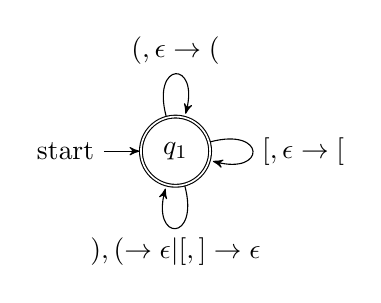
\begin{tikzpicture}
\node[state,accepting, initial] (q1) {$q_1$};
\draw 
(q1) edge[loop above] node{$(,\epsilon \rightarrow ($} (q1)
(q1) edge[loop right] node{$[,\epsilon \rightarrow [$} (q1)
(q1) edge[loop below] node{$),( \rightarrow \epsilon | [,] \rightarrow \epsilon$ } (q1);
\end{tikzpicture}

\section*{Question 5}
$S \rightarrow P | Q$  P for the case where $n\leq p$ and Q for $m \leq p$\\
$Q \rightarrow aQ | T$ Generates a for $m \leq p$ \\
$P \rightarrow aPc |Pc |R$  Generates a and c while making sure that $n \leq p$ \\ 
$R \rightarrow Rb | \epsilon$  Generates $b^*$  \\ 
$T \rightarrow bTc | Tc | \epsilon$  Generate b and c while making sure that $m \leq p$ \\

This language generates $\{a^nb^mc^p| n\leq p \lor m \leq p\}$
     

\section*{Question 6}
\subsection*{6.1}
We have a DFA $(Q,\Sigma, \delta, F, q_0)$ that recognizes the language L. 
We construct a left linear grammar $(N,\Sigma,S,P)$ using the DFA

Clearly, $\Sigma$ does not change and stays the same, $N=Q$, the set of states of the origional DFA, 
and for every trasition $\delta(P,\sigma) = Q$ we have the production $P \rightarrow \sigma Q$.
For every final state $Q \in F$ we have the production $Q \rightarrow \epsilon$
The start symbol is $S$, which is equivalent to $q_0$

\subsection*{6.2}
False.

Consider the following grammar $ S \rightarrow aSb|  \epsilon$
This clearly generates language $\{a^nb^n | n \in N\}$ which is not regular.

\section*{Question 7}
\subsection*{7.1}
If $i\neq j$ we stack all a till we reach a b, and we pop an a for each b.
If the stack is empty and we are not done reading bs then we move to an accept state and loop until we finish the string.
If we finish the b's and the stack is not empty then we still move to an accept state and otherwise we reject.
If $j \neq k$ we know that a and b are balanced, so we stack the bs and until we reach a c, then we pop a b for each c. Follow the same reasoning as we do for case $i \neq j$

\subsection*{7.2}
If it is a deterministic CFL, then the language's complement is a deterministic CFL as well, 
i.e $L'=\{a^ib^jc^k|i = j \land j = k\}$ is a deterministic CFL. 
However, such a language is not a CFL, therefore the initial PDA cannot be deterministic because of the closure principle.


\section*{Question 8}
It is clear that a regular language is a CFL, so we only need to show the other direction.

For an CFL $\Sigma=\{a\}$, there exist  $u,v,w,x,y \in \Sigma^* $such that $s=uvwxy, |vx|\geq 1, |vwx|\leq p$ and that $\forall i \geq 0, uv^iwx^iy \in L$ 

Here, $s= a^{n+m} \in L$ where $uwy=a^n,vx=a^m$ $1 \leq m\leq p$ and $uv^iwx^iy=a^{n+im} \in L, i\geq 0$

Suppose $L_0$ is a set of words with length less than p so it is finite and regular, and $L_m$ be the set of words with length greater than p 

$L=L_0 \cup \bigcup_{m=1}^{p}L_m$

If element $w \in L$ then either $|w|<p \lor |w| \geq p$ which means it is clearly a member of the union.

For any element $w \in RHS$ either it is in $L_0$ or $L_m$ or a pumped version, and are all in L.

Now we need to show that this is a finite union of regular languages. We need to show $L_m$ is regular for $1 \leq m\leq p$

$L_m =\{a^{n+im}| i \geq 0,a^{n+m} \in L_m\}$

Consider each $L_m$ we can partition it into sets $L_{m,s}$ of arithmetic sequences with difference between consecutive term m and starting term s (grouping by mod m).

$L_{m,s}=\{a^{|s|+(i-1)m}|i\geq 0\} = a^{|s|}(a^m)^*$

Each set is clearly regular, and there can be at most m disjoint sequences in $L_m$, so $L_m$ clearly regular.

So L is the finite union of regular languages and is also regular.



\section*{Question 9}
$L= \{a^nb^mc^mdde^{3n} | m,n \geq 1\}$ is context free as we can represent by the following grammar

$S\rightarrow aSeee|aTddeee$

$T\rightarrow bTC | bc$

Since $lefthalf(L) \cap \{a^*b^*c^*d\} = \{a^nb^nc^nd|n>0\}$, it is not context free because its intersection with a regular language is not context free.

\section*{Question 10}

\subsection*{10.1}
False.

The only way to check if an element is in the union is to check if it's in any of the sets individually,
but there is countably infinite sets so you won't halt if you're looking for an element that's not in the set.

\subsection*{10.2}
True.

Use dovetailing to output all element of the set so its computably enumerable. With dovetailing you will eventually list all elements of the sets even though there are countably infinitely many of them, and one definition of being computably enumerable is to have a way of listing all elements in the set. In other words, if you are looking for an element that does appear in the set you are guaranteed to find it eventually.




\end{document}
